\RequirePackage[hyphens]{url}

\documentclass[sigconf]{acmart}

\usepackage{tikz}

\makeatletter
\pgfdeclareshape{datastore}{
  \inheritsavedanchors[from=rectangle]
  \inheritanchorborder[from=rectangle]
  \inheritanchor[from=rectangle]{center}
  \inheritanchor[from=rectangle]{base}
  \inheritanchor[from=rectangle]{north}
  \inheritanchor[from=rectangle]{north east}
  \inheritanchor[from=rectangle]{east}
  \inheritanchor[from=rectangle]{south east}
  \inheritanchor[from=rectangle]{south}
  \inheritanchor[from=rectangle]{south west}
  \inheritanchor[from=rectangle]{west}
  \inheritanchor[from=rectangle]{north west}
  \backgroundpath{
    %  store lower right in xa/ya and upper right in xb/yb
    \southwest \pgf@xa=\pgf@x \pgf@ya=\pgf@y
    \northeast \pgf@xb=\pgf@x \pgf@yb=\pgf@y
    \pgfpathmoveto{\pgfpoint{\pgf@xa}{\pgf@ya}}
    \pgfpathlineto{\pgfpoint{\pgf@xb}{\pgf@ya}}
    \pgfpathmoveto{\pgfpoint{\pgf@xa}{\pgf@yb}}
    \pgfpathlineto{\pgfpoint{\pgf@xb}{\pgf@yb}}
 }
}
\makeatother




\usepackage{graphicx}
\usepackage{hyperref}
\usepackage{todonotes}

\usepackage{endfloat}
\renewcommand{\efloatseparator}{\mbox{}} % no new page between figures

\usepackage{booktabs} % For formal tables

\settopmatter{printacmref=false} % Removes citation information below abstract
\renewcommand\footnotetextcopyrightpermission[1]{} % removes footnote with conference information in first column
\pagestyle{plain} % removes running headers

\newcommand{\TODO}[1]{\todo[inline]{#1}}

\usetikzlibrary{arrows}

\begin{document}


\title{The Importance of Data Sharing and Replication, But What About Data Archiving?}




\author{J. Robert Langlois}
\affiliation{%
  \institution{Indiana University}
 \address{}
  \city{Bloomington, IN 47408} 
  \country{USA}}
\email{langloir@umail.iu.edu}




\begin{abstract}


With the increase of digital information, scientists have faced many challenges when it comes to the topic of big data management, including data archiving and data sharing. while it is unproblematic to share and archive quantitative data, qualitative data remains a puzzle that social scientists need to solve when it comes to what data to share, where to house the data, who will pay to store the data, how long the data should be kept for, etc. Many researchers are skeptical to engage in the practice of sharing digital information due to privacy concern, fear of stigmatization, the problem of funding, repository of data, transparency, and so forth. While it is important to keep these challenges in mind, it is critical to take a look at the different advantages of data sharing and data archiving.

\end{abstract}



\keywords{i523, HID325, Data Sharing and Data Archiving}


\maketitle


\section{Introduction}


Nowadays, many fields are witnessing a large influx of data due to the increase usage of technology. The digital data generated from scientific research is integral to the advancement of different scientific fields. While these data sets exist in abundant quantities, one challenge that many fields face is the lack of and/or prohibition of data being shared among researchers. Data sharing and its subsequent replication is a subject matter that is in dispute within in the sciences \cite{leetaru2016}. This is a significant area of contention in the United States; however, in other countries like the United Kingdom (U.K.), this issue has been addressed by making data sharing a matter of great importance; so much so, that the Joint Information Systems Committee of the U.K. made "data-sharing a priority, and has helped to establish a Digital Curation Centre…to be national focus for research and development into data issues" \cite{pryor2009skilling}. On one hand, opponents of data sharing are skeptical about this practice due to privacy concerns, fears of stigmatization, funding problems, repositories for data, transparency, etc. On the other hand, some researchers are open to data sharing because it allows their work to be reviewed and creates opportunities to further their findings; however, the actual practice is stunted by researchers concerns \cite{nelson2009empty}. Proponents of data sharing continue to advocate for an open access policy that would allow data to quickly respond to societal problems and crises, as well as advance the sciences. While it is as important to keep in mind the different challenges to data sharing, like data archiving, sharing data among fellow scientists can be very beneficial, not only can this practice help to maximize profits, make new discoveries, and respond to crises more quickly, but also it can play a vital role in advancing science and research.


\section{The Relevance of Data Sharing and Data Replication }



\subsection{ Define Big Data, Data Sharing, and replication}


Big data "is data that exceeds the processing capacity of traditional databases. The data is too big to be processed by a single machine. New and innovative methods are required to process and store such large volumes of data" \cite{gupta2014big}. The data sets are so voluminous and complex that traditional way of data processing application software are insufficient to deal with them. 

Data sharing can be understood as the ability to share research findings with multiple users. This technique implies that the digital information is being archived in one or multiple servers in the network and that there is other technique to prevent this information from being altered by two or more users at the same time. It is the practice of making data used for scholarly research available to other investigators. Data sharing is nothing but making the data available for other users to use for the common good of society. \cite{Datasharing}. 

Data replication is the process of copying data from one location to another. The technology helps an organization to possess up-to-date copies of its data in the event of a disaster."Replication can take place over a storage area network, local area network or local wide area network, as well as to the cloud. For disaster recovery (DR) purposes, replication typically occurs between a primary storage location and a secondary offsite location" \cite{Datarep2017}.


\subsection{The Advantages of Big Data}


we cannot talk about the advantages of Big data without quickly acknowledge that its numerous challenges, which include data collection, data storage, data analysis, search, sharing, transfer, visualization, etc. 

Big data analysis presents numerous advantages. For instance, it helps businesses to increase their productivity. This has done through a process of analyzing raw data that produces information that identifies trends and patterns that will help businesses make cost effective decisions. It is also helpful in aiding government agencies to improve public sector administration, and assists global organizations in analyzing information that has wide-reaching impact on the world. The information produced by big data can help medical professionals to detect diseases in earlier stages. Some other advantages of big data analysis is present in many different areas, such as:  smart grids, which monitor and control electricity use; traffic management systems, which provide information about transportation infrastructure likes roads and highways, mass transit, construction, and traffic congestion; retail by studying customer purchasing behavior to improve store layout and marketing; payment processing by helping to detect fraudulent activity, etc \cite{tene2012big}. Data is being collected everywhere due to the use of the internet; therefore, businesses and scientists are trying to make the maximum profits from it. Data sharing, for instance, can help scientist to respond to epidemic and crisis in a quickly manner. 


\subsubsection{Data Sharing Helps to Respond to Crisis Quicker}

Sharing data among fellow scientists and researchers is crucial. This process can help to respond to crisis quicker. By sharing (digital) data, researchers do not always have to start from scratch when they are responding to societal problems, such as medical epidemics, economic instability issues, natural disasters, etc.  As previously mentioned, an important aspect of data sharing is its ability to be used to respond to and help expeditiously resolve societal issues. As found in  \cite{yozwiak2015data}, data sharing is encouraged among fellow researchers and scientists to quickly respond to outbreaks. The authors centered their arguments around the rise of Ebola back in April 2015 that raised serious panic around the whole world due to the dangerous impacts of the disease that could result in death from just one exposure. They explained how the rapid availability of research data had facilitated a more amenable response time to the rapidly spreading threat of Ebola. The data accessed allowed it to be determined that the virus had circulated from Guinea to Sierra Leone and that it was being sustained by person-to-person contact. 

The fact that the data was recoverable from the GenBank, a public database, allowed researchers ready access and assisted with tracking the source of the deadly virus; thus, leading to the advocacy for the sharing of data among researchers to allow for quicker responses to life-threatening crises. This is one example of how data sharing can have a crucial impact on the response time researchers have when responding to disasters that have a global impact.

Moreover, \cite{vogel2014delays} wrote about the problem that public health policies faced when it came to responding to outbreaks like Ebola. He explained how bureaucracy and a lack of record keeping often delayed the ability of scientists to respond. A lack of collaboration among researchers can hinder progress when scientists need to respond to crises. Not only does data sharing help scientists to respond to and help provide critical solutions to outbreaks like Ebola, but access to the data can also contribute to the advancement of science through data replication. Thus, the importance to encourage this practice among fellow researchers. 

Certain research studies have supported the idea that big data allows for real time tracking of diseases and the development, prediction of outbreaks, and facilitates the development of personalized healthcare. Big data can also be used to maximize profits in many disciplines, including healthcare if harnessed properly \cite{van2011health}. "By harnessing big data, businesses gain many advantages, including increased operational efficiency, informed strategic direction, improved customer service, new products, and new customers and markets" \cite{khan2014big}. While data exists in huge quantities in many fields, including the health care field, individual privacy concerns remain a big problem that policymakers have to tackle to meet current trends in data collection. Improved methods of protecting very personal, private and sensitive health information is needed in order to allow for safe, necessary and adequate access to protected health information within the health care industry. Without proper policies related to data use, access, and protection, this big data potential can not be realized \cite{roski2014creating}. Data sharing and replication contribute to increase the availability of the amounts of digital information and make the access to information easier. 


\subsubsection {Data Sharing and Replication Contribute to Increase the Availability of Digital Information}

Furthermore, data sharing and replication (the availability of multiple copies of a data set to different users) is an important practice that plays a crucial role in the advancing of the sciences. The way sciences grow is through scaffolding, which means that one must rely on the work of previously published research to come up with new findings; thus, further supporting the necessity for a collaborative effort among researchers and scientists. Data sharing has been shown to help spot errors in research. In 2013, for example, a graduate student pointed out a calculation error made by two Harvard professors. This discovery was only possible because the professors shared a spreadsheet of their research findings with the particular student \cite{leetaru2016}. In this case, and possibly in many other cases, data sharing has helped to build community among fellow researchers, uncover honest mistakes and, in worst-case scenarios, expose possible fraud. Another researcher made a series of observations about the relevance of sharing data and asked many poignant questions regarding content, parameters and the necessity for sharing information. One observation she made was that "science progressed for centuries without data sharing policies and then questioned, why is data sharing deemed so important to scientific progress now?" \cite{borgman2015if}. She challenged the notion of free and unhindered distribution of data and cautioned that preliminary questions must first be answered to determine what data to share, how much and in what context data should be released to advance the changes in sciences. Her point was that the data should not stand alone, but rather it ought to be accurately defined and contextualized within the means that identified, developed and synthesized the data into usable information. While Borgman's scrutiny has its place in the argument regarding the absence of policies—which she argues ought to be based on accurately defining the data parameters—and their ability to facilitate data sharing, it is also important to acknowledge that the various scientific fields have been faced with different types of data and challenges. 

Nowadays, scientists are being bombarded with an abundant presence of digital data, which has made it difficult to manage and store, and far more difficult to compare data exchanges to what it was centuries ago. If digital data that is generated through research is not being replicated, the world of science will face far more challenges in the years ahead due to a lack of evolving data to build upon. Data replication involves open access to data so that researchers can continually study, analyze, and make new discoveries about existing data. Now, if data sharing opens the door to the replication of scientific research and advancement, then why is there so much opposition to such a practice? Without replication, the sciences may become stagnant in their advancement of theories and potential solutions to global problems. Not only data sharing makes access to information easier, but also helps to mitigate/eliminate unnecessary cost. 


\subsubsection{Data Sharing Help Reduce Unnecessary Cost
}

Another reason to encourage data sharing is that data sharing help to reduce unnecessary cost. As digital information is made available in the cloud system, researchers will be able to access the same type of information at different locations.  "Data sharing is driven by the need to maintain more accurate and up-to-date spatial databases, but at the same time reduce data acquisition and maintenance costs" \cite{stoakes2005data}. If data becomes more accessible, not only this will contribute to lowering the cost to access data, but also will it encourage researchers in their endeavors to respond to social outbreak quicker. Data sharing can also play a crucial role in advancing science, which is our next point. 

\subsubsection{Data Sharing Advances the Science}

Contrarily to what many might think, the advancement science occurs through replication of existing findings; scientists must rely on the work of previous researchers to make new discoveries. Just like human being cannot live in vacuum; the way science develop is through collaborative effort among fellow scientists."Placing research data online allows instantaneous access by a globally dispersed group of researchers to share, understand, and synthesize results. This aggregation and synthesis provide an opportunity for insight, progress, and that uniquely human quest for larger understanding. Data repositories also allow for the publication of previously hidden negative data, essentially experiments that didn't work" \cite{Uswyshyn2016}. One advantage of this practice is that by sharing their work, scientists will be able to spout errors that previous researchers have made, reveal fraud, build community, etc \cite{leetaru2016}. As found in \cite{borgman2012conundrum} policy makers must develop policies that explain how to embark in this process. If data are not being replicated, the world of science will face far more challenges in the future. Data replication involves open access to data so that researchers can continue to study, analyze, and make new conclusion about existing data. Now, if data sharing allows the replication of the sciences, why are many people opposed such practice? 


\section{Blocks to Data Sharing}

There are numerous barriers to data sharing. One of the barriers to data sharing is transparency. 


\subsection{Transparency Issue}

Some researchers fear that their work is going to be poached and that they will not get credit for their findings, so they hold on to it and do not disclose it. The concerns of obscurity and/or credit being assigned to other researchers who might advance the original researcher's findings will cause a serious reluctance to sharing data. As found in \cite{leetaru2016}, the term data parasites is used to describe the practice of utilizing data without giving proper credit to prior publishers. Thus, to overcome this challenge, there should be honesty and allowance for intellectual probity; a sort of fair play between researchers where appropriate credit would be given. In addition to giving appropriate credit for findings, another important aspect of disclosure is the appropriate compensation for the release of intellectual property. Oftentimes, researcher have sacrificed their time, income potential, energies, and relationships to do the work they do; incentive needs to be provided to encourage the sharing of their findings that they have worked hard to develop. "The call for transparency is not new, of course. Rather the emphasis is on access to data in a usable format, which can work to create value to individuals" \cite{tene2012big}. Access to digital information can engage individuals, invite scrutiny, and expose misuses of data. 

Another concern pointed out by this author is that data sharing may open the door for data analysts to disprove and/or scrutinize the work of the data producers. A potential solution that he proposed to this issue was co-authorship. He believed this would discourage the misuse of data by allowing collaboration among researchers \cite{leetaru2016}. Another researcher also asserted that researchers ought to agree on the standards of practice needed to responsibly share data. She advocated that both data and its means of publication deserve equal status in scholarly communications to determine how to cite data in non-trivial ways \cite{borgman2015if}. If data sharing and collaboration among researchers is to be effective, there need to be norms and regulations of how to do so. Collaboration among scientists can be a good thing to help mitigate and even eradicate the sense of fear that many researchers have in sharing their findings and the methodologies used to produce them. This leads us to our next potential block and challenge to data sharing, privacy concern. 


\subsection{The Problem of Individuals' Privacy}

Another barrier to data sharing, specifically in the healthcare field, involves the protection of patient privacy; a lack thereof can lead to stigmatization and potentially hamper patients’ participation in healthcare research and treatment. "Privacy is a major concern in outsourced data. recently some controversies have revealed how some security agencies are using data generated by individuals for their own benefits without permission. Therefore, policies that cover all user privacy concerns should be developed. Furthermore, rule violators should be identified and users data should not be misused or leaked" \cite{khan2014big}. In so doing, individuals will feel more at ease to engage in the process of sharing information for the benefits of everyone.


As \cite{yozwiak2015data} highlighted, some uncertainties that are involved data sharing, like whether data belongs to public or private domains. Still, another barrier is patient consent and their ability to fully understand how their participation can make them vulnerable to being potentially shunned and ostracized in their community based on their diagnosis and/or treatment. The researchers advocated for the responsible sharing of pertinent information among researchers to avoid this problem. It should also be mentioned that preclusion to the sharing of unnecessary information would also weaken the barriers to data sharing. Although data sharing is important, particularly during a medical outbreak, researchers ought to do their best to protect patient privacy to avoid any threat of stigmatization or isolation of patients. Rigorous ethical standards should be applied to safeguard patients' privacy and dignity to allow for easier sharing of relevant data \cite{yozwiak2015data}. Shelton (2011) advanced that "Rather than viewing privacy concerns as impediment, policy makers, scientists and HIT specialists should embrace privacy as an opportunity that, if addressed, can enhance the flow of information" \cite{shelton2011electronic}. If patients' privacy is protected, this will ease and mitigate skepticism within those who are refusing to share their personal information for fear that their privacy will be violated. These steps in the research process can facilitate the progression of scientific research through the increase of public participation and collaboration. 


Besides addressing privacy concerns, researchers can focus on understanding what aspects of data need to be preserved and dispensed for the public good. As another potential barrier, data preservation and the awareness of what data needs to be preserved raises concerns about data quality, the absence of scientists to analyze data, and data storage options. Funding for research needs to be contingent upon the determination of the importance of digital data. Policies ought to be developed that relate to the use of data, such as what data to be preserved as well as what exceptions need to be made to data preservation. In addition, regulations about data hosts (warehouses for storing data) should be determined. For example, "Agencies and the research community together need to create the digital equivalent of libraries: institutions that can take responsibility for preserving digital data and making them accessible over the long term" \cite{pryor2009skilling}.  Moreover, an effort to teach information management should be prioritized to facilitate data acquisition, data cleansing, data storage, and effective uses of data. While most scientific disciplines found that a data deluge is extremely challenging, great opportunities can be realized with better organization and open access to data \cite{economic22challenges}. It is important to train scientists, establish better policies to regulate data sharing, and increase the incentives for researchers from every fields to collaborate as they tackle the many issues that are faced by the modern sciences.


For data sharing and replication to be effective, scientists from diverse fields ought to come together because very rarely can progress happen in isolation. Currently, very few fields like astronomy, genomics, social sciences, and archaeology practice data sharing. The lack of success in implementing data sharing policies conveys the need for greater understanding of the roles of data in various sciences; highlighting the need to also seek the development of new models of scientific practice \cite{borgman2015if}. A new model can be in the arena of archiving; archiving data can be very expensive and difficult to manage, thus while it is encouraging that scientists share their work with each other, it is also crucial to have serious conversation about data housing, and the financial responsibility that involves in this practice. Until researchers come together to satisfy the response to those barriers, data sharing will remain a challenge among scientists. And if today's scientists and researchers do not make the effort to work together to facilitate effective and essential data sharing, future generations will experience the problem of lost data due to a lack of effective stewardship. 


\subsection{Ways to Overcome Privacy Concern}


Three types of data are being identified: 1. personal and proprietary data, which are controlled by individuals and non-government organizations; 2. government controlled data, which includes, for instance, personal tax, census data, and personal health records; and finally, open data commons, which are available to everyone to access and use. The author advocated for policy makers develop strategy to link personal, proprietary, and government data to pursue health care care objectives \cite{van2011health}. When we think about privacy concerns it is crucial to see collaboration between scientists from different sectors. By working together they will be more equipped to develop policies that can help to mitigate the risk of data leaking.

One way policymakers can protect individual privacy is by making the data anonymous. Researchers have identified three types of data: personal and proprietary data that is controlled by individuals; government-controlled data, which government agencies can restrict access to; and, open data commons, which means that the data is centrally located and available to all. Big data analysts and researchers have advocated for linking data together that can help to improve health care planning at both the patient and population levels. They also argued for an increase in the amount of information that is available in open data commons \cite{roski2014creating}. Although the anonymization of data appears to be a great technique that policymakers could espouse to address privacy concerns, other studies have indicated that some data can be traced back to their respective individual; thus, destroying the argument for anonymity \cite{van2011health}.  "Every copy of data increases the risk of unintended disclosure. To reduce this risk, data should be anonymized before transfer; upon receipt, the recipient will have no choice but anonymize it at rest...And re-identification is by design, in order to ensure accountability, reconciliation and audit" \cite{cavoukian2012privacy} If proper norms are established for data analysis, this can potentially contribute to improvements in the health care industry, and businesses can maximize profit from it. 


\subsubsection{Privacy Principles and Data Architecture}


Privacy principles should be introduced during the process of data architecture; privacy should be incorporated into the design and operational procedures \cite{cavoukian2012privacy}. In so doing, personal health care data, for example, will be protected against malicious hackers who try to access individuals' personal health information for the purposes of stealing individuals' identity. Another type of data that has been introduced to the healthcare industry is concept quantified self data. It can be understood as the data produced by individuals that engage in self-tracking of personal health information, such as heart rate, weight, energy levels, sleep quality, cognitive performance, etc. These individuals use devices like smart-phones, watches, and wearable technology sensors in the collection of their personal data and biometrics. It has been shown that 60 percent of U.S. adults are tracking their weight, diet or exercise routines, while 33 percent are monitoring their blood sugar, blood pressure, sleep patterns, etc. This indicates that there is a vast amount of health information that has been produced by individuals. What is done with all of this data? This massive supply demonstrates the need to develop policies and protocols that involve individual patient consent to share their collected data; this data can be critical to the advancement of health-care with the support of data analysis. Before that can be done; however, we must first establish the proper norm to use this type of data so that the privacy of individuals can be protected; this ought to be the primary action to take \cite{swan2013quantified}. Because many individuals are willing to collect information about themselves without being prompted to do so; this is a good sign that is proper norm is established around data management and incentive is given to encourage data sharing, individuals will be willing to engage in the process of sharing their personal data. Although it is often complicated to share qualitative data, the challenge to share seems to increase when dealing with healthcare data. 

In the healthcare industry, Patients often do not want their health information to fall in the hand of other entities without their consent; however, with proper informed consent, patients seemed to become willing to share their personal health information.As agencies work with patients to disclose the purposes of collecting certain, sometimes sensitive, health information, they can empower patients to make informed decisions about their personal health information, thus engaging patients in the process. This can then serve to increase and improve the set of personal health information utilized for clinical research purposes, and subsequently improve people's lives \cite{shelton2011electronic}. 
"Privacy concerns exist wherever personally identifiable information or other sensitive information is collected and stored in any form" \cite{khan2016digital}. Thus, to protect privacy, other techniques, like encryption, authentication, and data masking may be utilized to ensure that the information is available only to authorized users.


\section{Saving Scientific Data for Future Generations}


\subsection{Data Archiving}

Along with the conversation surrounding data sharing and replication, another important conversation that needs to take place is around the infrastructure needed to archive data. While many people engage in a debate to encourage data sharing among scientists, the infrastructure to preserve the data does not yet fully exist. In reference to data, Nelson (2009) drew on a proverbial question, is it the chicken or the egg; what comes first, data sharing or the space to store data? He contends that while data sharing is encouraged among scientists, the infrastructure to store data is nonexistent and it is arduous task to pursue the development of it \cite{nelson2009empty}. Thus, it is tantamount to talk about data saving as we encourage data sharing because if scientists resort to sharing their findings then there also need to be a safe place to house the data. This preservation is critical for future generations to build upon the work that has already been done to advance scientific research. As the advocacy for data archiving increases, a new challenge arises: who will pay for all of this?

\subsubsection{Who Should Pay to Store the Data?}


Serious conversation needs to continue to happen around data management. "Access to data requires that the data be hosted somewhere and managed by someone" \cite{berman2013will}. Although they acknowledged the effort of public and private sectors to archive data in certain fields like the life sciences, they also stipulated that many federally funded research data are at risk due to the lack of long-term structure that can ensure continual access and preservation of data. If data are not housed well, it could be said that a lot of efforts, money, and energies, are being wasted away due to lack of a secure and sustaining system of storage. As found in \cite{lynch2008big}, the author posited that scientists are not the best stewards of data and suggested the job of data archiving be entrusted to the institutions that employ the researchers. Ensuring that data is well preserved will lay the important groundwork for allowing data to be accessible in the future. Lynch also emphasized the idea that for data saving to be effective, collaboration between funders, institutions and scientists are crucial. He gave the example, such as the GenBank and the U.S.'s National Institutes of Health (NIH) genetic sequence database, as well as the U.S. National Virtual Observatory, to show the possibilities of what can be done. It appears that collaboration between sectors is key when it comes data management, including data archiving. It is not the job of one sector, but it is the job of all of us. Only when all of the sectors converge their effort together, we will be able to respond the quandary of Big data management. 

Some researchers proposed four approaches that can help improve the partnership among sectors: 1) incentivize the private sector to be stewards of public research, 2) utilize the power of partnership between the public and private sectors to fund viable solutions, 3) create clear policies for the management of public data, and finally 4) encourage openness to new and diverse methods of research to advance public research abilities. Furthermore, they theorized that there should be adequate safeguards to prevent private sector’s control, access and use of public data \cite{berman2013will} . While these measures are applicable, there not be all great because by relinquishing the work of data saving to the private sector solely, it can create a very expensive problem to accessing data via private organizations that are highly incentivized by financial gains. It would probably be more effective if the federal government would pay for their own data scientists to be trained on how to effectively manage the data, and establish the requirements and expectations that all federally funded research remains in the public domain. 


Other research corroborates the idea of licensing all research data to the public domain. This is the case, in the Netherlands, where for example, all the data retrievals are kept by the National Library. The U.S. can espouse this model by creating a center for data to be stored, and develop policies on how to access the data. This would prevent the private sector from having a monopoly on accessing, interpreting, sharing and store data that belongs in the public domain \cite{sarkol2016scientific}.  Another researcher advanced and noted that, in its effort to encourage peer review, the National Science Foundation (NSF), makes data sharing a requirement in the grant contract, where researchers are required to submit a 2-page report of their research that can be used to facilitate peer review. This technique used by NSF was revealed to be a great example of how the federal government can overcome the conundrum of data sharing and archiving among scientists \cite{borgman2012conundrum}. This technique is applicable, however, proper norm stills to be established and proper security measure needs to be created to preclude the data leaking, which can compromise the privacy of research participants.


\subsection{Electronic Versus Physical Archives}


Another conversation that needs to happen when it comes to Big data management is how to archive the data. Scientists need to decide between electronic archiving versus physical archiving. "Digital archives face specific challenges linked to physical storage media as well as hardware and software longevity. In reality, every method of recording information, whether on paper, stone, or photographic film, has a limited resistance to time. The value of any information is dependent on the ability to decode it after a long storage period. The difference with digital archives is that these limits are ignored because of the addition of complex and versatile technology to the overall equation" \cite{stamatiadis2005digital}. Thus, it is important that researchers figure out which form they want to espouse to archive that will allow long term access to the data. It can be argued that both forms have its advantages and disadvantages. Physical archiving allows access to the data locally and no sophisticated knowledge or programming skills are needed to access the data; however, the data is not available everywhere; this form of archiving data is quite limited. On the other hand, electronic archiving allows multiple users to access the data at the same time. It can be said that the digital information is not limited to physical location and space; the data is located in the cloud; it is unbound and can be accessed from everywhere. "The advantages of a digital archive in the pharmaceutical sector cover four areas: accessibility, selectivity, fidelity, and compliance" \cite{stamatiadis2005digital}.

The only disadvantage to digital information is probable the lack of skills to access and manipulate the data. "As we move into the electronic era of digital objects, it is important to know that there are new barbarians at the gate and that we are moving into an era where much of what we know today, much of what is coded and written electronically, will be lost forever. We are, to my mind, living in the midst of digital Dark Ages; consequently, much as monks of times past, it falls to librarians and archivists to hold to the tradition which reveres history and the published heritage of our times" \cite{stamatiadis2005digital}. Thus, the necessity to continue to train more data scientists and analysts who can extract, manipulate, and analyze the information from the cloud system.  

\section{Train New Scientist to Help to Manage data}

If we are talking about data sharing, data replication and data archiving, it is critical to address the how to do so? The skills to extract, collect, and store data have not been taught yet in regular school. If we want to develop a generation of data driven society, we need to start teaching computer skills in elementary school all the way to college and university. Just like we teach natural language, like English, French, Spanish to children at a very young age, it is important to teach programming language skills to these kids, so that we can increase their awareness and develop incentive to become data analysts, scientists who will be able to manipulate the data sets. There is an old proverbial that states that " You can teach an old dog new tricks." Thus, the earlier we start teaching those skills, the better.  While there are many institutions that have shown interest in developing Data Scientists by teaching programming language skills, like python, java, C++, machine learning, data analysis, etc. so that data can be extracted and analyzed, it would be great to start teaching programming skills to students at a lower level, like elementary school. The same way certain math skills like probability has been taught in high school, it is relevant to start incorporating programming language skills in high school to develop interest and incentive to engage in the process of collecting, manipulating, and housing digital information.

 
\subsection{Why Data Repository?}


Data repository facilitates access to existing documents. "Besides being a good thing for the sharing and verification of data-driven research results, data research repositories are now necessary for university campuses. Placing one’s research data online has become mandatory for any researcher wishing to receive grants from any public U.S. agency. This includes the National Institutes of Health (NIH), National Science Foundation (NSF), U.S. Department of Agriculture (USDA), and National Endowment for the Humanities (NEH). The rational is that if a researcher is drawing from the public taxpayers’ trough, the research must be publicly accessible through both the article and original data. Sharing this data helps keep the wider economy vital, facilitating healthy competition toward commercialization and dissemination of discovery. If researchers do not have data management plans in place, their chance of obtaining a grant decreases. Currently, a majority of grant-funded researchers do not share data. With recent mandated changes, this situation is rapidly changing. Ivy League institutions have already capitalized on it—sharing data leverages and enhances faculty, departmental, and a university’s global research standing" \cite{Uswyshyn2016}. If research data is made available, this can contribute to lessen and even mitigate the stress level of graduate students when they work on dissertation and final project for their respective institutions. Not only it would save them the time to go to different libraries to hunt for documents to start working on their project, but also it gives them access to all the work that has been done on the topic chosen, and what else is left to be done. 


Data repositories can play a vital role in making research findings available to everyone and making access to data an easy process. "Online research data repositories are large database infrastructures set up to manage, share, access, and archive researchers' datasets. Repositories may be specialized and relegated to aggregating disciplinary data or more general, collecting over larger knowledge areas, such as the sciences or social sciences. Online repositories may also aggregate experts' data globally or locally, collecting a university or consortium of universities researcher's data for mutual benefit. The simple idea is that sharing data improves results and drives research and discovery forward. A repository allows examination, proof, review, transparency, and validation of a researcher's results by other experts beyond the published refereed academic article. Placing research data online allows instantaneous access by a globally dispersed group of researchers to share, understand, and synthesize results. This aggregation and synthesis provide an opportunity for insight, progress, and that uniquely human quest for larger understanding. Data repositories also allow for the publication of previously hidden negative data, essentially experiments that didn't work. This enables other researchers to avoid previous dead ends of those who have tried a path before them to better find their way toward more fertile territory" \cite{Uswyshyn2016}. 


\section{Figure}

The following data flow diagrams convey the flow of information in a system. This  figure shows experimental data being collected, reported, processed and stored \cite{fokkema2012}. This figure is depiction, an example of how data management works. The data go through a series of process before it can be archived and reused. 

As we can see, management big data requires that highly individuals to collect, clean, analyze, store, and share the data. it is not the work of one individuals; it is the work of all of us. We more data analysts who can engage in analyzing the data; we need more data collectors to collect and create raw data and spreadsheets to be analyzed; we need more individuals who can create structures and security around data storing, etc. It was never the work of one individual, all of us need to be involved. 

Thus, it is critical to converge our effort in passing the management tools and skills to current students and developing scientists who will be highly skilled in managing Big data analysis. Considering all of the different breakthroughs that are happening in the digital realm, it is safe to say that Big data is bigger and bigger; thus the necessity to train scientists to face the challenges that await us ahead.





\begin{center}
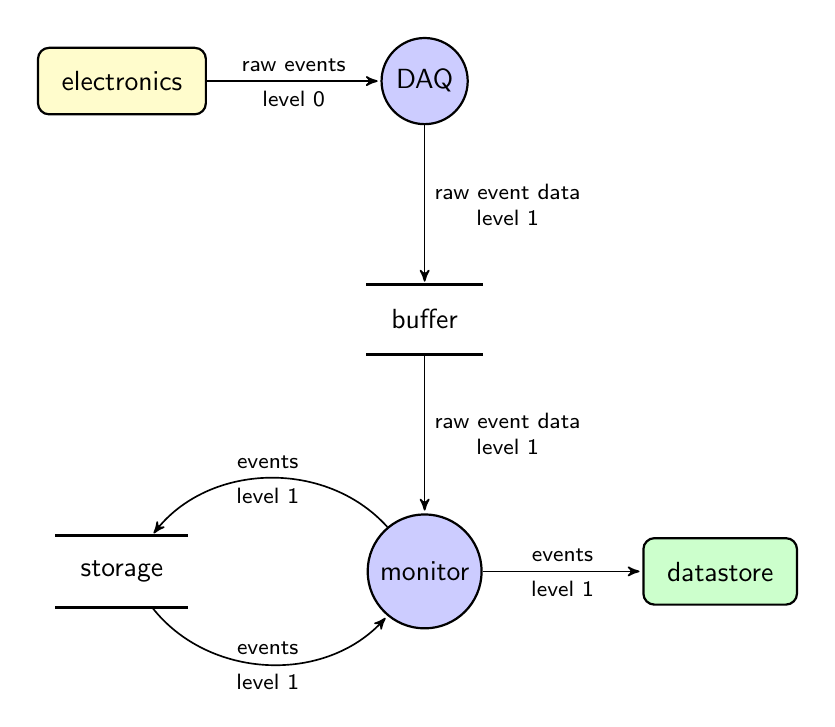
\begin{tikzpicture}[
  font=\sffamily,
  every matrix/.style={ampersand replacement=\&,column sep=2cm,row sep=2cm},
  source/.style={draw,thick,rounded corners,fill=yellow!20,inner sep=.3cm},
  process/.style={draw,thick,circle,fill=blue!20},
  sink/.style={source,fill=green!20},
  datastore/.style={draw,very thick,shape=datastore,inner sep=.3cm},
  dots/.style={gray,scale=2},
  to/.style={->,>=stealth',shorten >=1pt,semithick,font=\sffamily\footnotesize},
  every node/.style={align=center}]

  % Position the nodes using a matrix layout
  \matrix{
    \node[source] (hisparcbox) {electronics};
      \& \node[process] (daq) {DAQ}; \& \\

    \& \node[datastore] (buffer) {buffer}; \& \\

    \node[datastore] (storage) {storage};
      \& \node[process] (monitor) {monitor};
      \& \node[sink] (datastore) {datastore}; \\
  };

  % Draw the arrows between the nodes and label them.
  \draw[to] (hisparcbox) -- node[midway,above] {raw events}
      node[midway,below] {level 0} (daq);
  \draw[to] (daq) -- node[midway,right] {raw event data\\level 1} (buffer);
  \draw[to] (buffer) --
      node[midway,right] {raw event data\\level 1} (monitor);
  \draw[to] (monitor) to[bend right=50] node[midway,above] {events}
      node[midway,below] {level 1} (storage);
  \draw[to] (storage) to[bend right=50] node[midway,above] {events}
      node[midway,below] {level 1} (monitor);
  \draw[to] (monitor) -- node[midway,above] {events}
      node[midway,below] {level 1} (datastore);
\end{tikzpicture}
\end{center}


\subsection{figure2}

\subsubsection{A simple Example of Data lifecycle}

This data lifecycle was created by Jerome Tremblay and is adapted to explain the different phases that the data take before it can be destroyed \cite{fokkema2012}.

The following figure is a depiction of the data lifecyle. The data often follows a number of steps, which are: in 1 we have (data creation), followed by 2 (data maintenance), 3 (data utilization), 4 (data publication), 5 (data archiving) and 6 (data destruction). In phase 1, the data gets created. Spreadsheets are often used by companies to keep the data. In this active process, the data is often stored locally on a server or multiple servers, or in the cloud, or a host data center. In phase 2, the data is data gets processed and synthesized in a variety of tasks. This is a fairly broad range of management actions, such as how data is supplied to the end users and how analytics such as modeling are performed on the data. In phase 3, the data is ready to be used by end users. In this phase the challenge of data governance and data compliance arise. In phase 4, the data can be published. In phase 5, the data is archive: At some point in time, the data in your system will have no immediate use, and it’s time to archive it in case it might be needed in the future. This removes the data from your active environment and moves it off to storage. In phase 6, When the data is no longer useful and needed, it must be destroyed. In this phase of the data lifecycle governance and compliance challenge might be surfaced. It’s important to ensure that the data has actually been destroyed properly for several reasons, among those reason to make sure that privacy of individuals are protected. Briefly, these are the difference phases that data take before it falls into desuetude. 

It is important to note that there are other types of data lifecycle in the realm of big data management that follow different stages, such as: data collection, in the this stage large amounts of raw data is being created;this stage is a significant aspect in the management of big data because it helps to capture the data that will later transition from raw data to published data. The second stage is data filtering and classification, in the stage the data is being filtered, cleaned and structured to eventually be ready to be analyzed. In the third stage, that data is ready to be analyzed. certain techniques and technologies are being used in the process of analyzing the data, such as data mining algorithm, cluster, correlation, statistical regression, indexing, graphics. Visualization and interpretation of the information happen in this very stage. The next stages that the data are storing, sharing, and publishing. After the data is being analyzed, the data is store for future use. "Data and its resources are collected and analyzed for storing, sharing, and publishing to benefit audiences, the public, tribal governments, academicians, researchers, scientific partners, federal agencies, and other stakeholders (e.g. industries, communities, and the media). Large and extensive Big data datasets must be stored and managed with reliability, availability, and easy accessibility, storage infrastructures must provide reliable space and a strong access interface that can not only analyze large amounts of data, but also store, manage, and determine data with relational DBMS structures. Storage capacity must be competitive given the sharp increase in data volume; hence, research on data storage is necessary" \cite{khan2014big}. Thus, the importance to develop good policies that will address privacy and different challenges that involves storing and sharing Big data for the benefits of every sectors. 

The codes for this figure was borrowed from Jerome Tremblay.


\begin{tikzpicture}

\def \n {6}
\def \radius {3cm}
\def \margin {8} % margin in angles, depends on the radius

\foreach \s in {1,...,\n}
{
  \node[draw, circle] at ({360/\n * (\s - 1)}:\radius) {$\s$};
  \draw[->, >=latex] ({360/\n * (\s - 1)+\margin}:\radius) 
    arc ({360/\n * (\s - 1)+\margin}:{360/\n * (\s)-\margin}:\radius);
}
\end{tikzpicture}


\section{Conclusion}

This document put forth the dialogue needed to assist researchers to address the different challenges they have experienced when it comes to data sharing and replication as well as data saving. The advantages and disadvantages of Big data analysis have been discussed. We have seen that though Big data applications has its advantages, it has its poses many challenges as well. The importance of data sharing has been explored, and examples of how sharing information can help scientists to respond to global crises in a timely manner, like in the Ebola outbreak, have been provided. It has also been shown how data sharing and replication have helped to advance scientific research. It was postulated that in order for data to continue to exist, scientists need to embrace the idea of replicating their information. 

As research continues to occur and scientists increase their agreement to collaborating with one another, they will be better equipped to discover potential errors from previous retrievals, fix those errors and clean the data, and make other discoveries based on existing data. Scientists cannot operate as an Island. Policies need to be put in place, to understand what data to share, when to share, where to store the data, and what data to store etc. For the continued advancement of the sciences, data sharing and archiving will require resources that facilitate the access, interpretation and maintenance of data. The importance of data sharing, data replication, and data archival cannot be overlooked. This work is far from exhaustive, More discussion around data management need to happen; new policies and regulations regarding how to share, store and replicate data  are needed as well as effective parameters for how these processes will be funded and used in the future.



\begin{acks}

  Thank you to Dr. Gregor von Laszewski for his support and suggestions to write this paper, and most importantly for teaching us how to use latex to write documents. This is a very important tool that everyone need to procure. It is very handy. From now on, latex is the new tool to write paper and article. I am so grateful for this class. Although I do not have any programming language background, being able to use latex to write documents is a big deal. I do not regret at all that I chose to take this course. It was a pleasure to be in this class. I have learned a lot in the course. I will definitely recommend this course to other students. Despite my meager python and programming skill, with the assistance of the TAs and the professor, I was able to respond to the challenge of this class. Thus, thank you so much everyone for your help and assistance .  

\end{acks}

\appendix

\bibliographystyle{ACM-Reference-Format}

\bibliography{report}

\end{document}
